\chapter{Ridge estimation of network models from time-course omics data \\ {\footnotesize(\textit{Miok, V., Wilting, S. M. and van Wieringen, W. N., Submitted for publication})}}
\chaptermark{{\tt ragt2ridges} package}
\label{chapter:Window estimator}

\graphicspath{{Chapter4/Figs/}{Chapter4/Figs/PDF/}{Chapter4/Figs/}}%


\section{The VAR(2) model}
\begin{figure}[h!]
\centering
\begin{tabular}{cc}
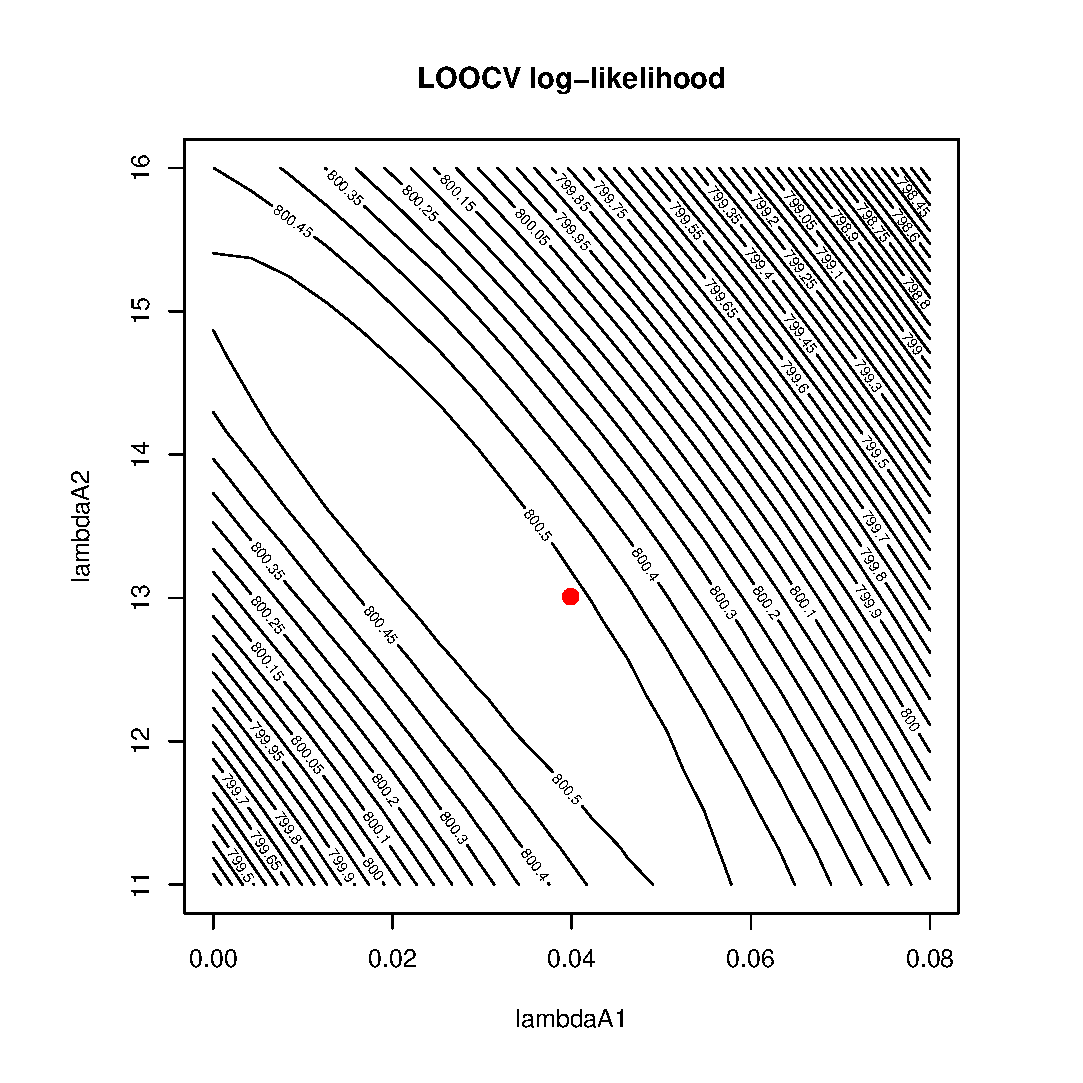
\includegraphics[scale=0.35]{Figure_5a.eps}
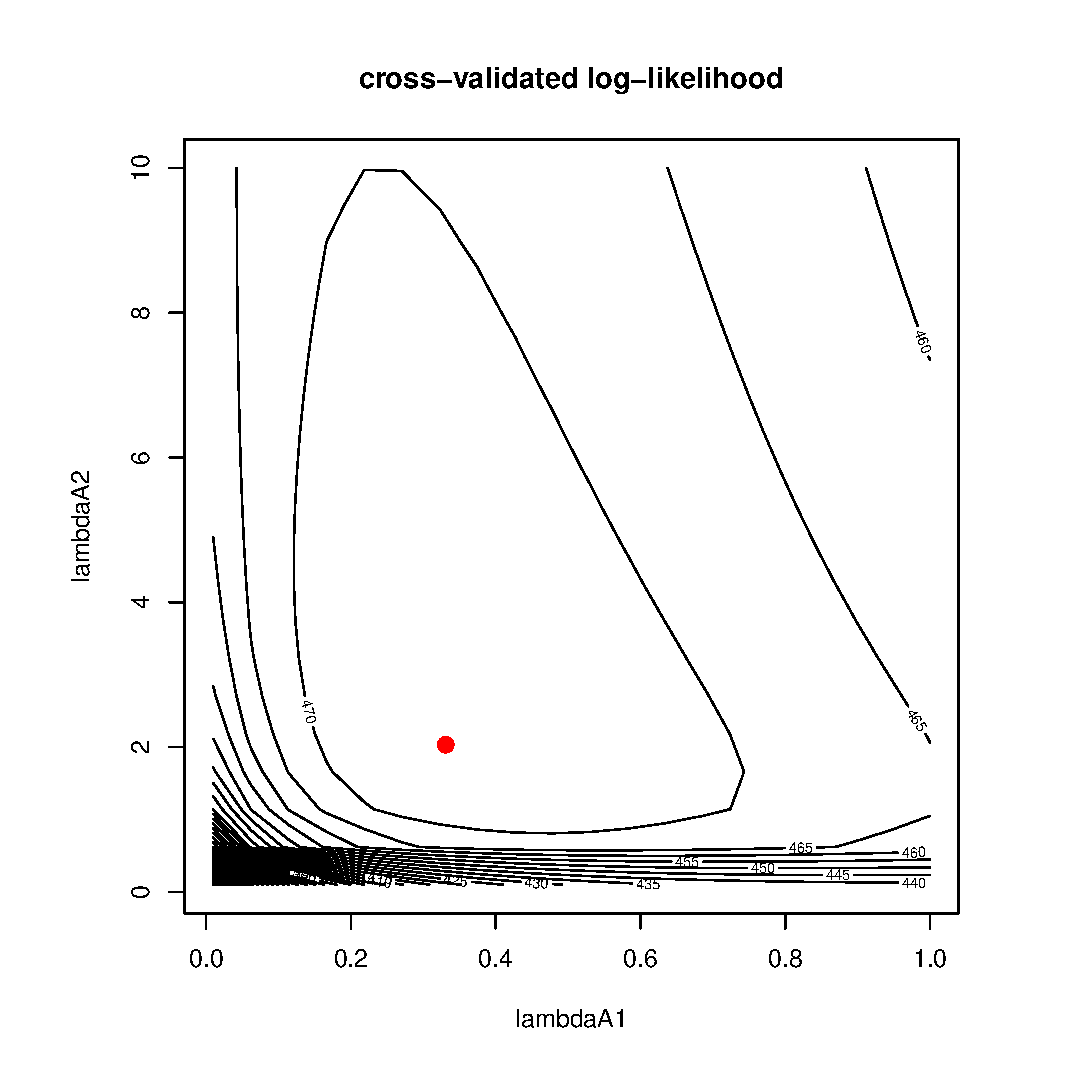
\includegraphics[scale=0.35]{Figure_5b.eps}
\end{tabular}
\caption{Contourplot of the VAR(2) LOOCV log-likelihood vs. the penalty parameters. Left and right panels show these contour plots of the situation with full and sparsified support, respectively.}
\label{fig:contourVAR2}
\end{figure}

\begin{figure}[h!]
\centering
\begin{tabular}{c}
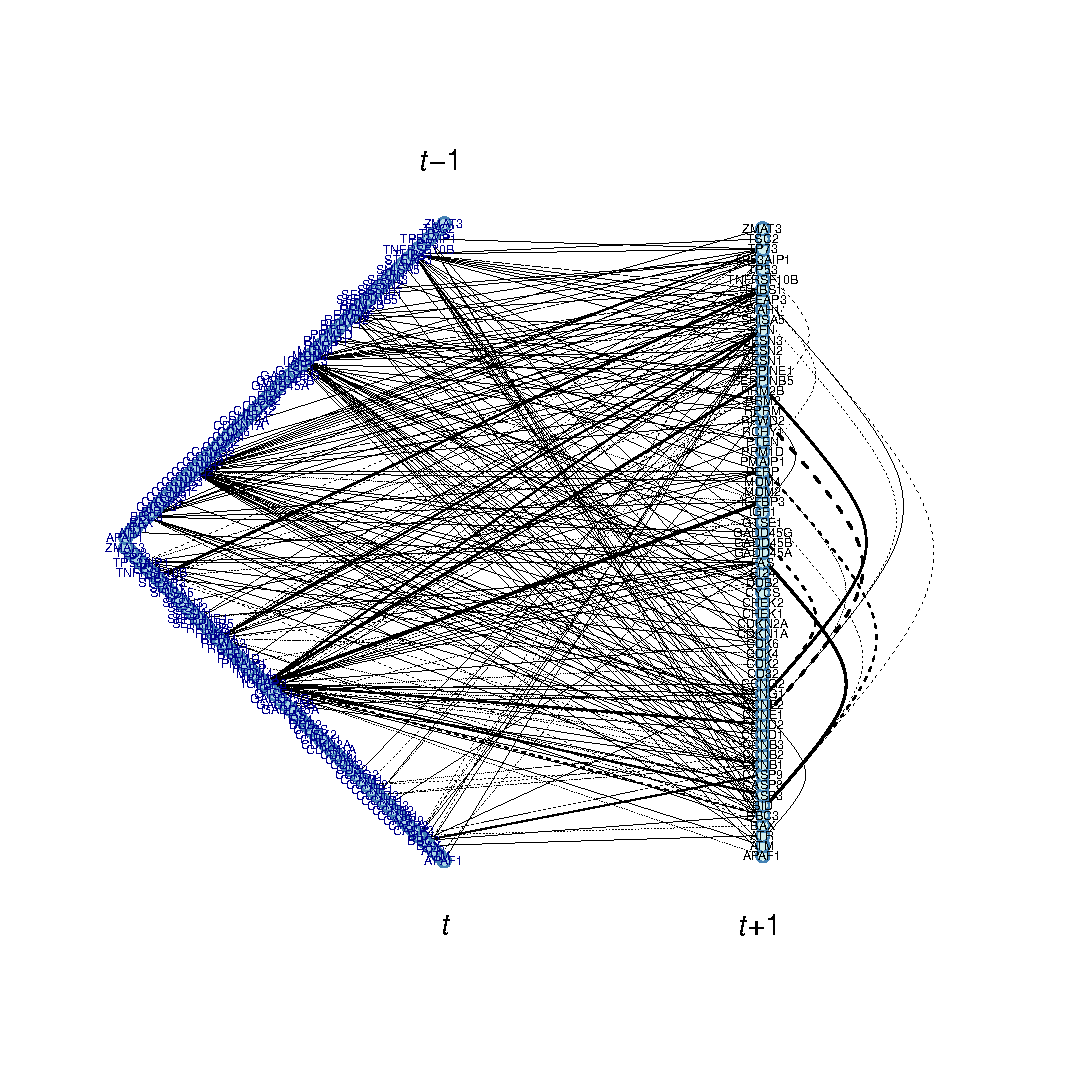
\includegraphics[scale=0.6]{Figure_6.eps}
\end{tabular}
\caption{Inferred time-series chain graph from the VAR(2) model. Solid and dashed lines represent a positive and negative relations, respectively. The thickness of the lines indicates the strength of the relation. Unconnected nodes have been pruned from the graph.}
\label{fig:graphVAR2}
\end{figure}


\newpage
The mutual information between $Y_{j,i,t}$ and $\mathbf{Y}_{\ast,i,t+\tau}$ (given $\mathbf{Y}_{*,i,t-\tau}$ for $\tau \in \mathbb{N}$) is defined as:
\begin{eqnarray*}
& & \hspace{-1cm} \mathcal{I}(\mathbf{Y}_{\ast,i,t+\tau},Y_{j,i,t}|\mathbf{Y}_{*,i,t-1},\mathbf{Y}_{*,i,t-2}) \, \, \, = \, \, \,
\\
& & \mathcal{H}(\mathbf{Y}_{*,i,t+\tau} \, | \, \mathbf{Y}_{*,i,t-1},\mathbf{Y}_{*,i,t-2}) - \mathcal{H}(\mathbf{Y}_{*,i,t+\tau} \, | \, Y_{j,i,t},\mathbf{Y}_{*,i,t-1},\mathbf{Y}_{*,i,t-2}),
\end{eqnarray*}
where $\mathcal{H}(\cdot|\cdot)$ is the (conditional) entropy. Under normality the entropy equals, e.g.:
\begin{eqnarray*}
H(\mathbf{Y}_{\ast,t+\tau,i} \, |  \, \mathbf{Y}_{\ast,t-1,i},\mathbf{Y}_{*,i,t-2})  \, \, \, = \, \, \, \textrm{log}(|\mathbb{V}(\mathbf{Y}_{\ast,t+\tau, i} \, | \, \mathbf{Y}_{\ast,t-1,i}, \mathbf{Y}_{\ast,t-2,i})|).
\end{eqnarray*}
For the VAR(2) model this variance is given by the following recursive relations:
\begin{eqnarray*}
& & \hspace{-1.0cm}  \mathbb{V}(\mathbf{Y}_{\ast, t + \tau, i} \, | \, \mathbf{Y}_{\ast, t -1, i}, \mathbf{Y}_{\ast, t -2, i}) \, \, \,  = \, \, \,  \mathbf{\Sigma}_{\varepsilon}
\\
& & + \mathbf{A}_1 \mathbb{V}(\mathbf{Y}_{\ast, t + \tau -1, i}  \, | \, \mathbf{Y}_{\ast, t -1, i}, \mathbf{Y}_{\ast, t -2, i}) \mathbf{A}_1^{\top}
\\
& & + \mathbf{A}_2 \mathbb{V}(\mathbf{Y}_{\ast, t + \tau -2, i}  \, | \, \mathbf{Y}_{\ast, t -1, i}, \mathbf{Y}_{\ast, t -2, i}) \mathbf{A}_2^{\top}
\\
&  & + \mathbf{A}_1 \mbox{Cov}(\mathbf{Y}_{\ast, t + \tau -1, i}, \mathbf{Y}_{\ast, t + \tau -2, i}  \, | \, \mathbf{Y}_{\ast, t -1, i}, \mathbf{Y}_{\ast, t -2, i}) \mathbf{A}_2^{\top}
\\
&  & + \mathbf{A}_2 \mbox{Cov}(\mathbf{Y}_{\ast, t + \tau -2, i}, \mathbf{Y}_{\ast, t + \tau -1, i}  \, | \, \mathbf{Y}_{\ast, t -1, i}, \mathbf{Y}_{\ast, t -2, i}) \mathbf{A}_1^{\top},
\\
& & \hspace{-1.0cm}
\mbox{Cov}(\mathbf{Y}_{\ast, t + \tau, i}, \mathbf{Y}_{\ast, t + \tau-1, i} \, | \, \mathbf{Y}_{\ast, t -1, i}, \mathbf{Y}_{\ast, t -2, i}) \, \, \, = \, \, \,
\\
&  & \mathbf{A}_1 \mathbb{V}(\mathbf{Y}_{\ast, t + \tau -1, i}  \, | \, \mathbf{Y}_{\ast, t -1, i}, \mathbf{Y}_{\ast, t -2, i})
\\
& & + \mathbf{A}_2 \mathbb{V}(\mathbf{Y}_{\ast, t + \tau -1, i}  \, | \, \mathbf{Y}_{\ast, t -1, i}, \mathbf{Y}_{\ast, t -2, i}) \mathbf{A}_1^{\top}
\\
&  & + \mathbf{A}_2 \mbox{Cov}(\mathbf{Y}_{\ast, t + \tau -2, i}, \mathbf{Y}_{\ast, t + \tau -3, i}  \, | \, \mathbf{Y}_{\ast, t -1, i}, \mathbf{Y}_{\ast, t -2, i}) \mathbf{A}_2^{\top}.
\end{eqnarray*}
The following initiations complete these recursive relations:
\begin{eqnarray*}
\mathbb{V}(\mathbf{Y}_{\ast, t, i} \, | \, \mathbf{Y}_{\ast, t -1, i}, \mathbf{Y}_{\ast, t -2, i}) & = & \mathbf{\Sigma}_{\varepsilon}
\\
\mathbb{V}(\mathbf{Y}_{\ast, t + 1, i} \, | \, \mathbf{Y}_{\ast, t -1, i}, \mathbf{Y}_{\ast, t -2, i}) &  = &  \mathbf{\Sigma}_{\varepsilon} + \mathbf{A}_1 \mathbf{\Sigma}_{\varepsilon} \mathbf{A}_1^{\top}
\\
\mbox{Cov}(\mathbf{Y}_{\ast, t, i}, \mathbf{Y}_{\ast, t -1, i} \, | \, \mathbf{Y}_{\ast, t -1, i}, \mathbf{Y}_{\ast, t -2, i}) & = & \mathbf{0}_{pp},
\\
\mbox{Cov}(\mathbf{Y}_{\ast, t+1, i}, \mathbf{Y}_{\ast, t, i} \, | \, \mathbf{Y}_{\ast, t -1, i}, \mathbf{Y}_{\ast, t -2, i}) & = & \mathbf{A}_1 \mathbf{\Sigma}_{\varepsilon},
\\
\mbox{Cov}(\mathbf{Y}_{\ast, t+2, i}, \mathbf{Y}_{\ast, t +1, i} \, | \, \mathbf{Y}_{\ast, t -1, i}, \mathbf{Y}_{\ast, t -2, i}) & = & \mathbf{A}_2 \mathbf{\Sigma}_{\varepsilon} \mathbf{A}_1^{\top} + \mathbf{A}_1 \mathbf{\Sigma}_{\varepsilon} + \mathbf{A}_1^2 \mathbf{\Sigma}_{\varepsilon} \mathbf{A}_1^{\top}.
\end{eqnarray*}
Rests that of the other entropy term, the evaluation of
$\mathbb{V}(\mathbf{Y}_{\ast,t+\tau, i} \, | \, Y_{j,t,i}, \mathbf{Y}_{\ast,t-1,i}, \mathbf{Y}_{\ast,t-2,i})$ employs the same recursive relations (also conditioning on $Y_{j,t,i}$ leaves them unaffected for $\tau > 2$). The initiations however change:
\begin{eqnarray*}
\mathbb{V}(\mathbf{Y}_{\ast, t, i} \, | \,  Y_{j,t,i}, \mathbf{Y}_{\ast, t -1, i}, \mathbf{Y}_{\ast, t -2, i}) & = & \mathbf{\Sigma}_{\varepsilon | j}
\\
\mathbb{V}(\mathbf{Y}_{\ast, t + 1, i} \, | \,  Y_{j,t,i}, \mathbf{Y}_{\ast, t -1, i}, \mathbf{Y}_{\ast, t -2, i}) &  = &  \mathbf{\Sigma}_{\varepsilon} + \mathbf{A}_1 \mathbf{\Sigma}_{\varepsilon |j } \mathbf{A}_1^{\top}
\\
\mathbb{V}(\mathbf{Y}_{\ast, t + 2, i} \, | \,  Y_{j,t,i}, \mathbf{Y}_{\ast, t -1, i}, \mathbf{Y}_{\ast, t -2, i}) &  = &  \mathbf{\Sigma}_{\varepsilon} + \mathbf{A}_1 \mathbf{\Sigma}_{\varepsilon } \mathbf{A}_1^{\top} + \mathbf{A}_2 \mathbf{\Sigma}_{\varepsilon |j } \mathbf{A}_2^{\top} + \mathbf{A}_1^2 \mathbf{\Sigma}_{\varepsilon |j } (\mathbf{A}_1^{\top})^2
\\
\mbox{Cov}(\mathbf{Y}_{\ast, t, i}, \mathbf{Y}_{\ast, t -1, i} \, | \,  Y_{j,t,i}, \mathbf{Y}_{\ast, t -1, i}, \mathbf{Y}_{\ast, t -2, i}) & = & \mathbf{0}_{pp},
\\
\mbox{Cov}(\mathbf{Y}_{\ast, t+1, i}, \mathbf{Y}_{\ast, t, i} \, | \,  Y_{j,t,i}, \mathbf{Y}_{\ast, t -1, i}, \mathbf{Y}_{\ast, t -2, i}) & = & \mathbf{A}_1 \mathbf{\Sigma}_{\varepsilon | j},
\\
\mbox{Cov}(\mathbf{Y}_{\ast, t+2, i}, \mathbf{Y}_{\ast, t +1, i} \, | \,  Y_{j,t,i}, \mathbf{Y}_{\ast, t -1, i}, \mathbf{Y}_{\ast, t -2, i}) & = & \mathbf{A}_2 \mathbf{\Sigma}_{\varepsilon | j} \mathbf{A}_1^{\top}
+ \mathbf{A}_1 \mathbf{\Sigma}_{\varepsilon} + \mathbf{A}_1^2 \mathbf{\Sigma}_{\varepsilon |j } \mathbf{A}_1^{\top},
\end{eqnarray*}
in which $\mathbf{\Sigma}_{\varepsilon | j} =
(\mathbf{\Sigma}_{\varepsilon})_{\setminus j, \setminus j} - (\mathbf{\Sigma}_{\varepsilon})_{\setminus j,j}[(\mathbf{\Sigma}_{\varepsilon})_{j,j}]^{-1} (\mathbf{\Sigma}_{\varepsilon})_{j,\setminus j}$, the covariance of the all but the $j$-th innovations conditional in the $j$-th one.

\newpage
\begin{table}
\caption{Node statistics for the top five 'regulators' and 'regulatees' (as derived from the time-series chain graph of the p53 signaling pathway) identified from the HPV16 affected cell line data using the VAR(2) model. For these genes, names in the left most column, the following node statistics are evaluated: the in- and out-degree of the lag-one temporal dependencies; the in- and out-degree of the lag-two temporal dependencies; the mutual information between the expression level of the gene at time $t$ and all other genes at time $t+2$ from the pathway and impulse response on the  the expression level of the gene at time $t$ and all other genes at time $t+2$.}
\begin{tabular}{l*{8}{c}r}
\hline
\hline          
             & $\mbox{deg}^-(\mathbf{A}_1)$ & $\mbox{deg}^+(\mathbf{A}_1)$  & $\mbox{deg}^-(\mathbf{A}_2)$ & $\mbox{deg}^+(\mathbf{A}_2)$  & mutual info. & impulse resp.  \\
\hline
IGFBP3       & 2 & 18 & 5 & 27 & 0.54358 & 0.02826 
\\
IGF1     & 1 & 18 & 0 & 10 & 0.05431 & 0.01213
\\
RPRM     & 4 & 17 & 2 & 10 & 0.19450 & 0.00799
\\
CCND2     & 2 & 4 & 5 & 32 & 0.05297 & 0.01623
\\
THBS1     & 3 & 8 & 6 & 20 & 0.17556 & 0.01143
\\
\\
SFN    & 8 & 0 & 5 & 0 & 0.00000 & 0.00000
\\
CCNB1        & 8 & 0 & 4 & 0 & 0.00000 & 0.00000
\\
TP73       & 3 & 0 & 8 & 0 & 0.00000 & 0.00000
\\
SESN2  & 3 & 0 & 4 & 0 & 0.00000 & 0.00000
\\
DDB2    & 2 & 0 & 4 & 0 & 0.00000 & 0.00000
\\
\hline
\end{tabular}
\label{table:postEstVAR2}
\end{table}

\mbox{ }

\newpage
\section{Multiple VAR(1) models}
\begin{figure}[h!]
\centering
\begin{tabular}{cc}
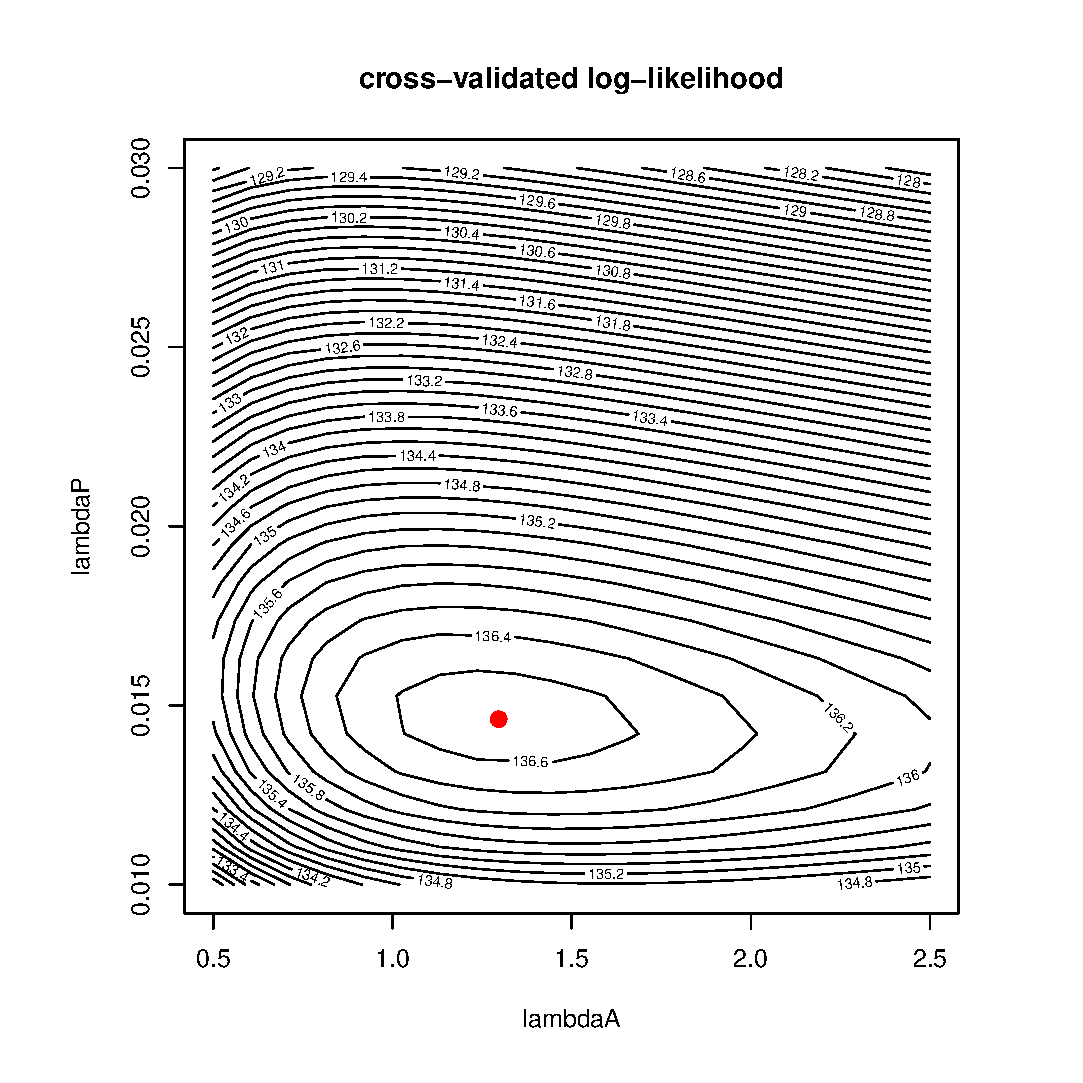
\includegraphics[scale=0.35]{Figure_9a.eps} &
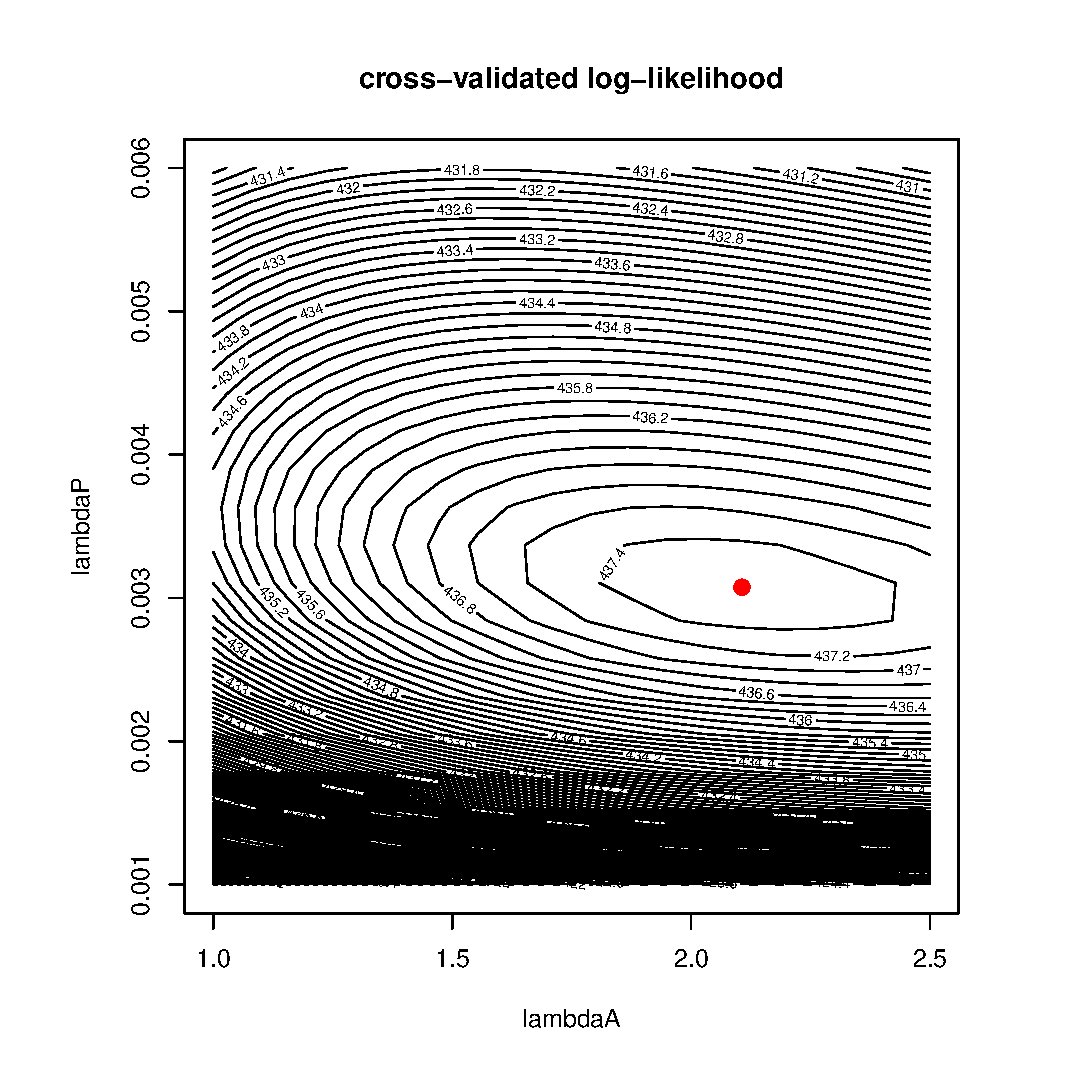
\includegraphics[scale=0.35]{Figure_9b.eps}
\end{tabular}
\caption{Contourplot of the multiple VAR(1) LOOCV log-likelihood vs. the penalty parameters. Left and right panels show these contour plots of the data from cell lines affected with HPV16 and HPV18, respectively.}
\label{fig:contourVAR2}
\end{figure}

\[
\]

\begin{figure}[h!]
\centering
\begin{tabular}{cc}
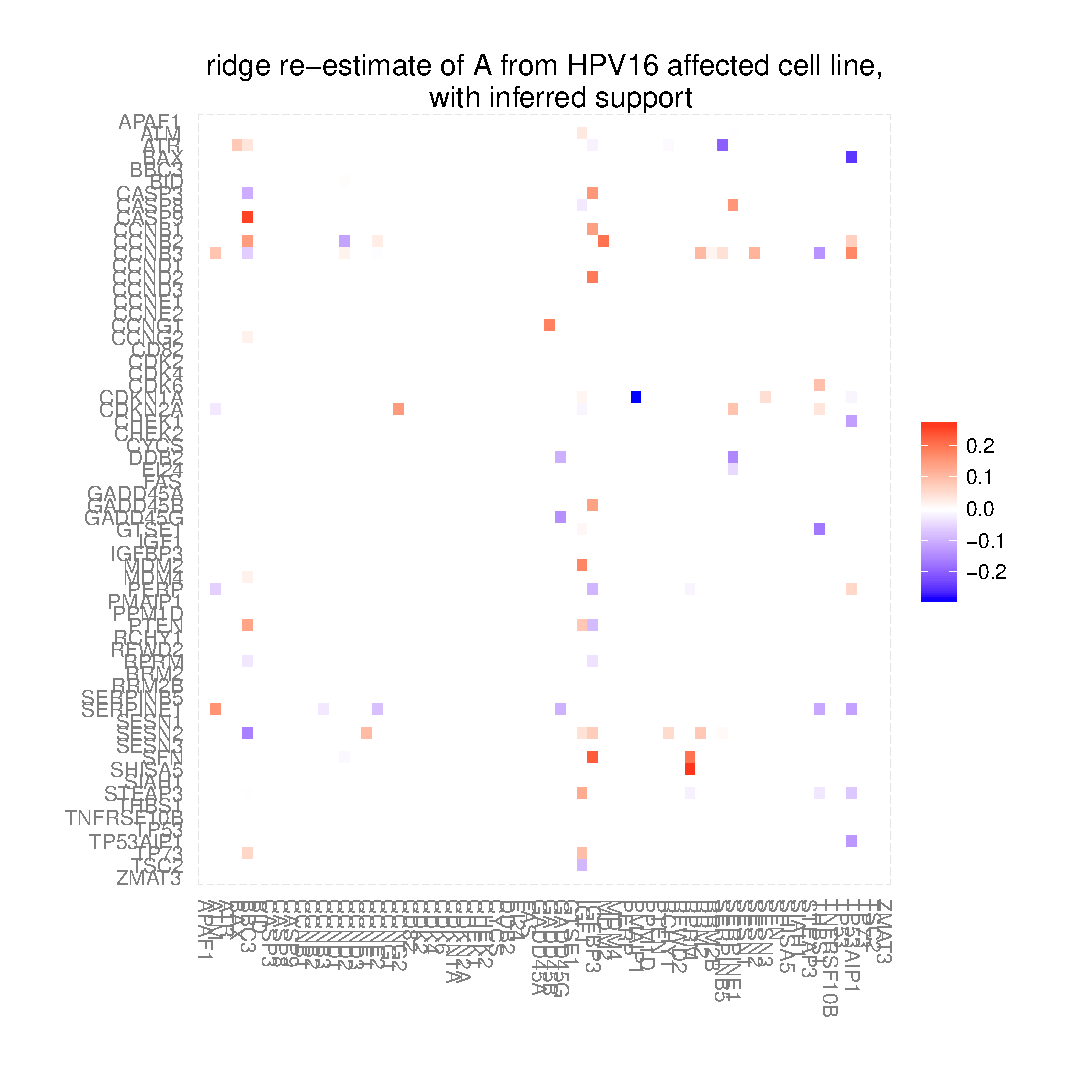
\includegraphics[width=2.9in, height=2.5in]{Figure_10a.eps}
&
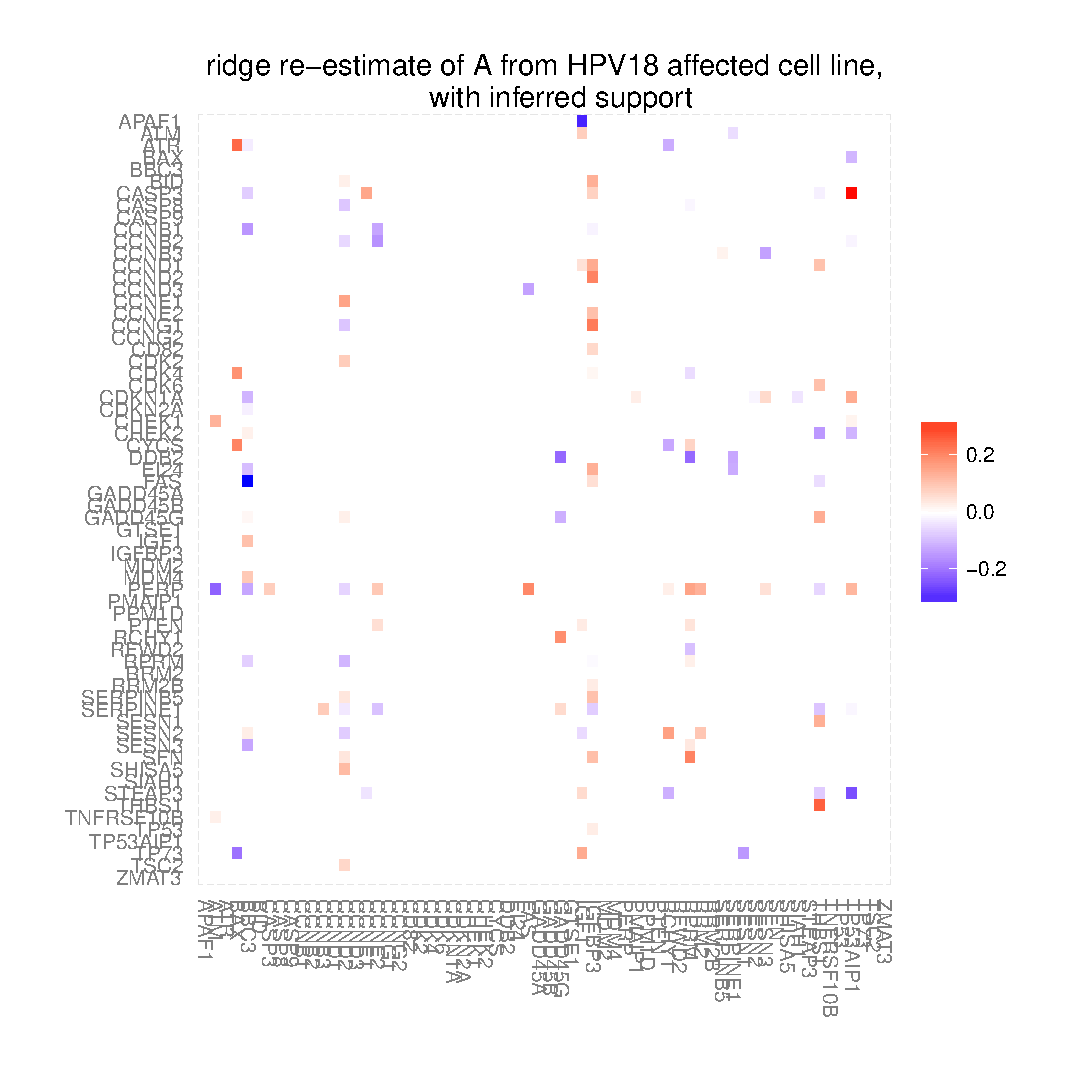
\includegraphics[width=2.9in, height=2.5in]{Figure_10b.eps}
\end{tabular}
\caption{Heatmaps of the sparsified re-estimated multiple VAR(1) model parameters. Left and right panel represent temporal interactions among mRNAs in the cell lines affected with HPV16 and HPV18, respectively.}
\label{fig:VARmultipleEst}
\end{figure}

\[
\]


\begin{figure}[h!]
\centering
\begin{tabular}{cc}
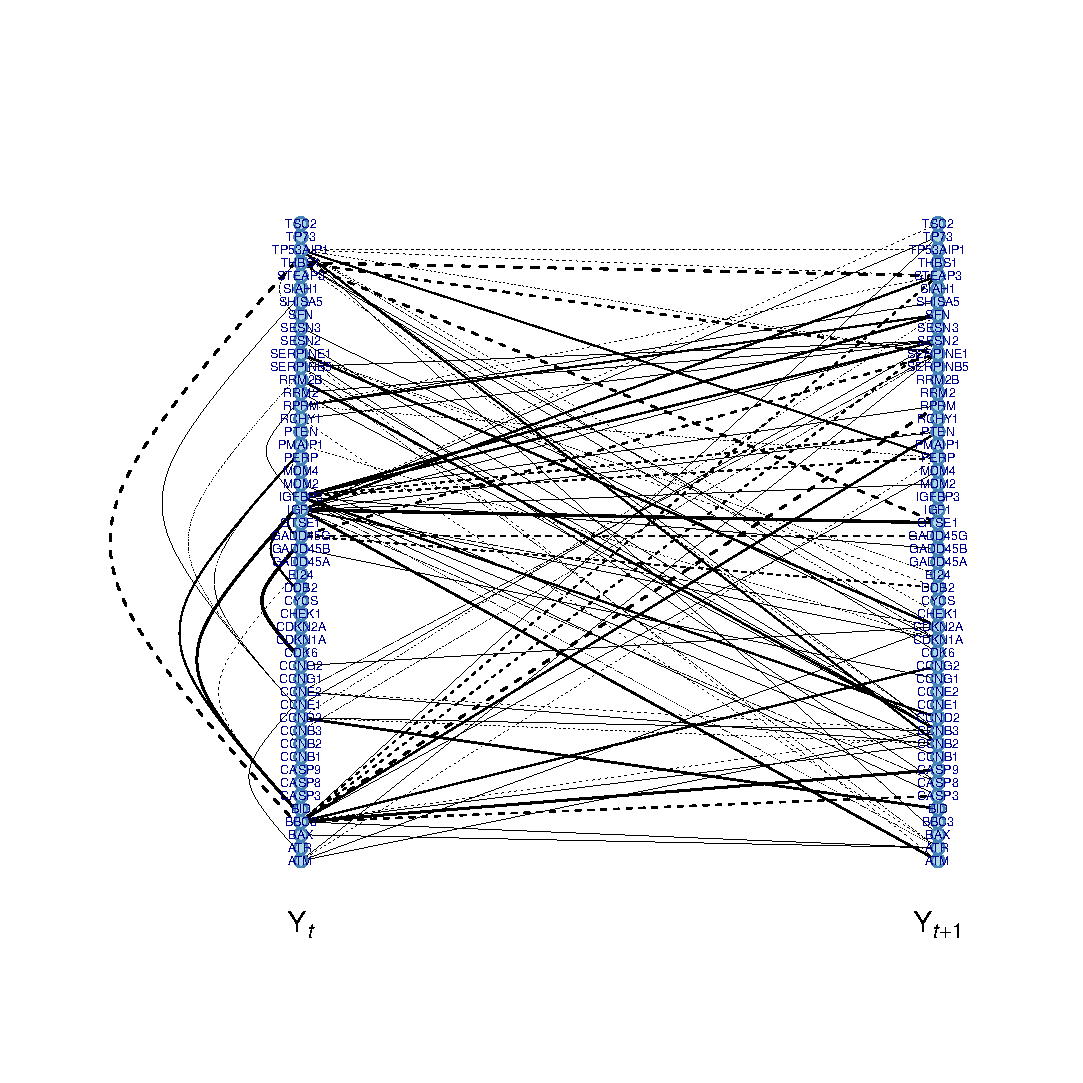
\includegraphics[scale=0.4]{Figure_11a.eps} &
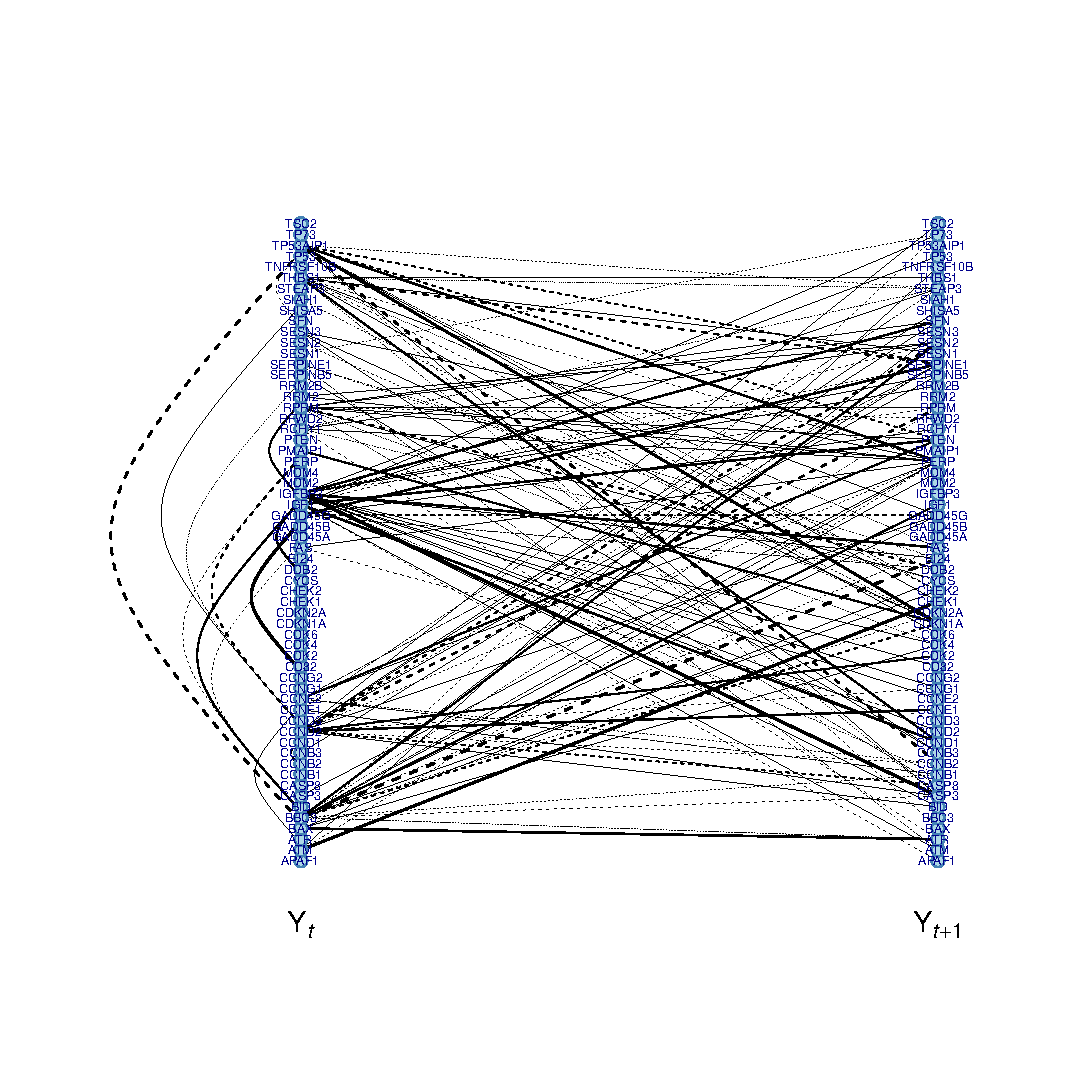
\includegraphics[scale=0.4]{Figure_11b.eps}
\end{tabular}
\caption{Left and right panels depict the inferred time-series chain graph from the cell lines affected with HPV16 and HPV18, respectively. Solid and dashed lines represent positive and negative relations, respectively. The thickness of the lines corresponds to the strength of the relation. Unconnected nodes have been pruned from the graph.}
\label{fig:graph}
\end{figure}

\[
\]
\newpage
\mbox{ }
\newpage
\section{The VARX(1) model} 
\begin{figure}[h!]
\centering
\begin{tabular}{cc}
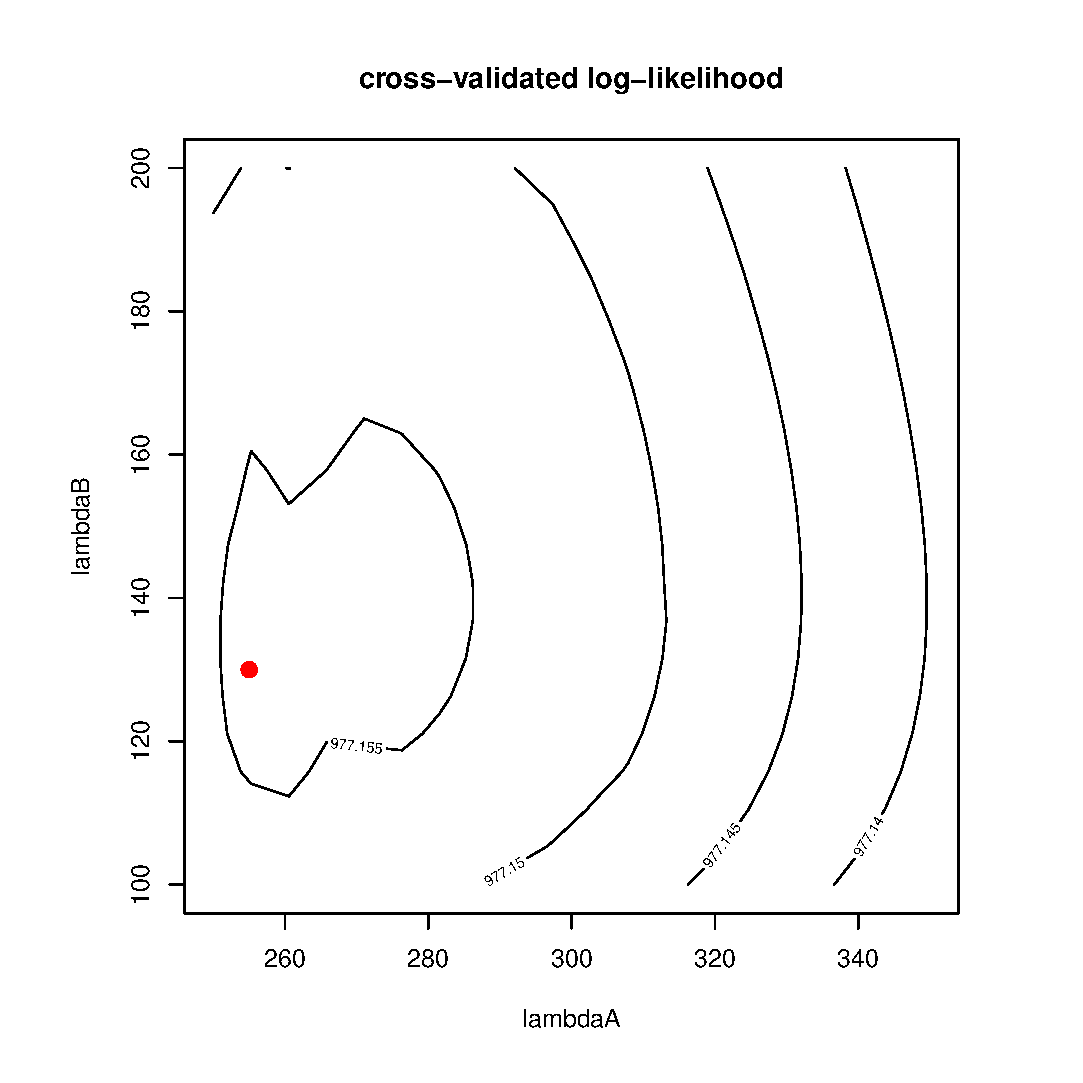
\includegraphics[scale=0.4]{Figure_15a.eps}
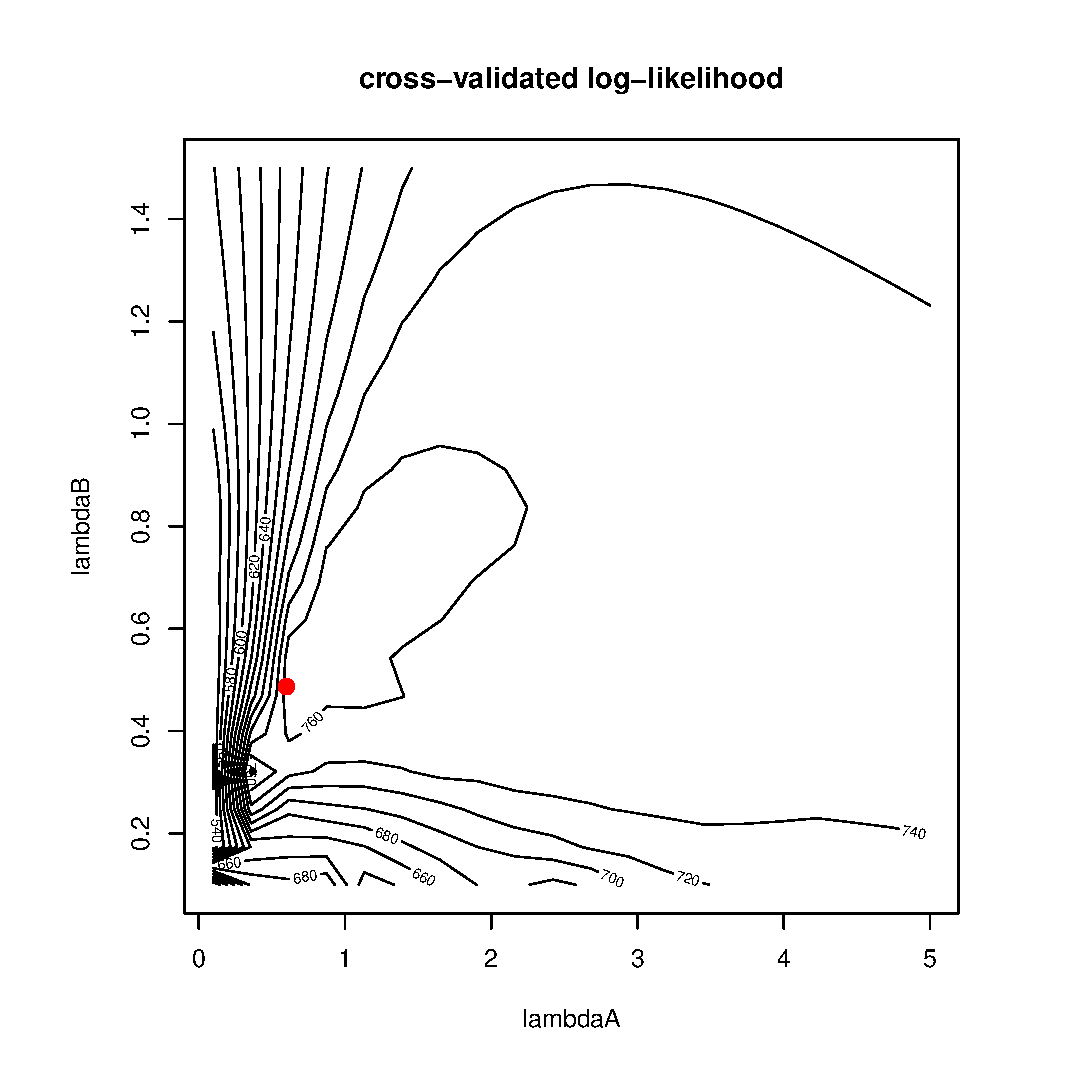
\includegraphics[scale=0.4]{Figure_15b.eps}
\end{tabular}
\caption{Contour plots of LOOCV log-likelihood vs. penalty parameters of the VARX(1) model. Left and right panels display the contour plots without and with inferred support, respectively.}
\label{fig:contourVARX}
\end{figure}


\begin{figure}[h!]
\centering
\begin{tabular}{cc}
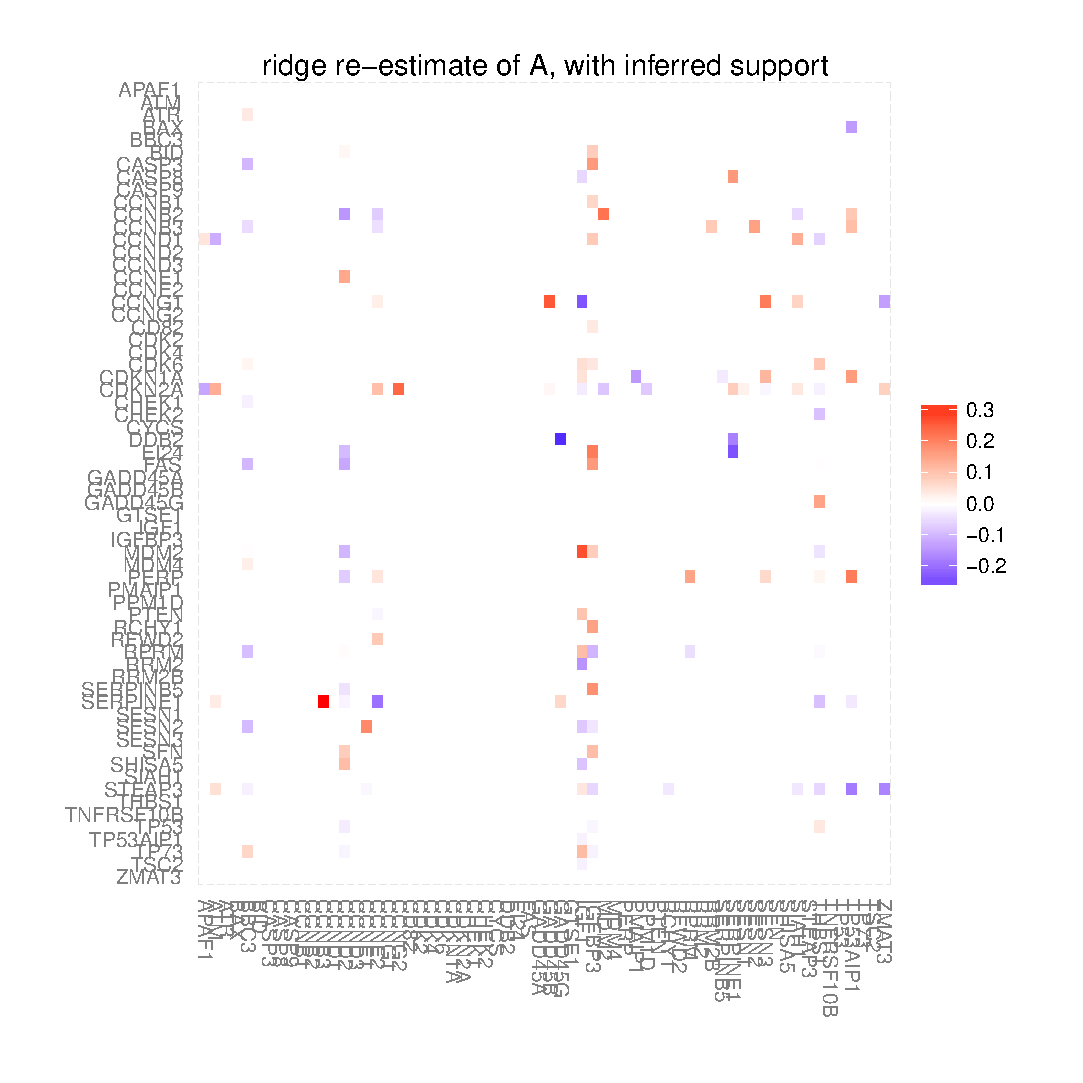
\includegraphics[scale=0.28]{Figure_16a.eps}
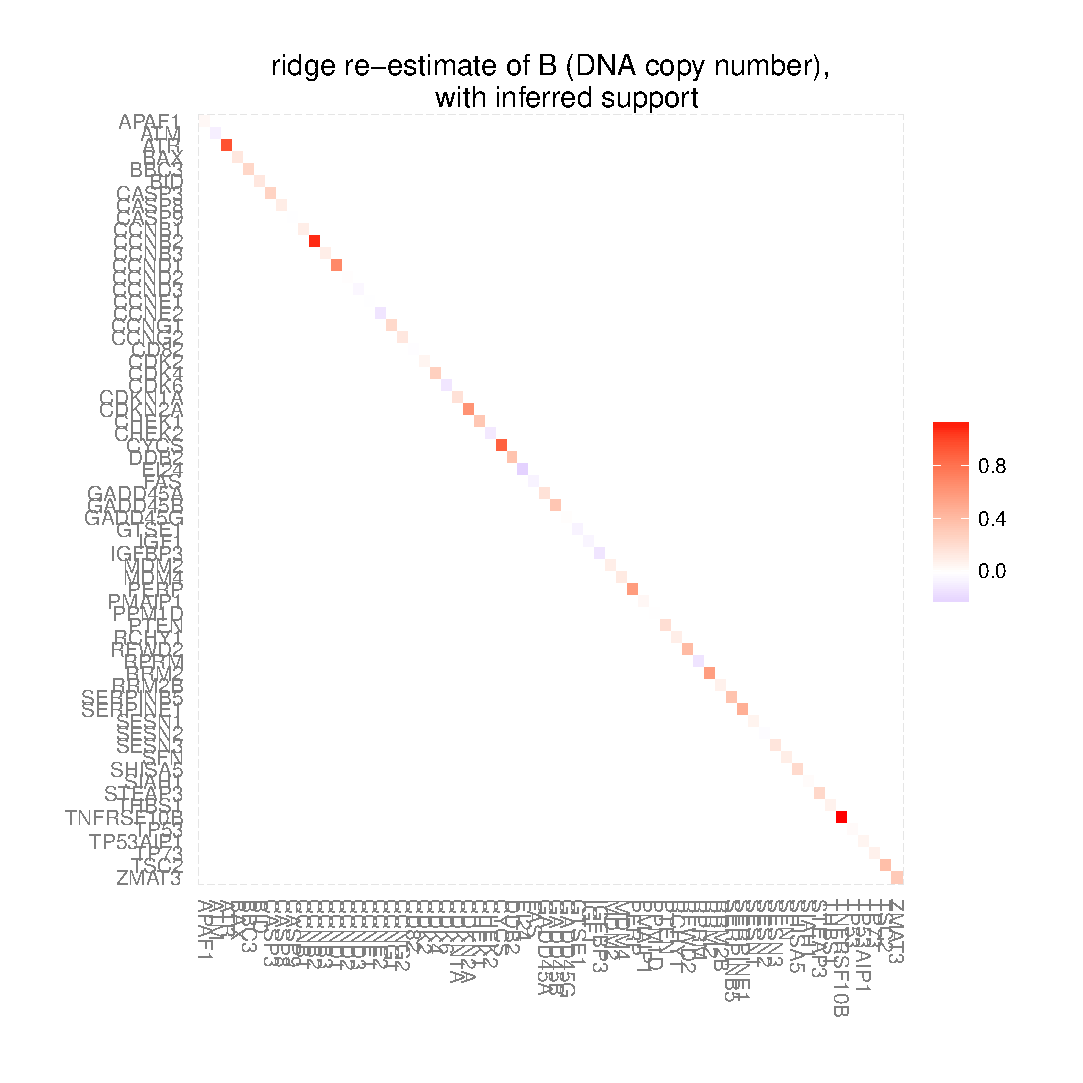
\includegraphics[scale=0.28]{Figure_16b.eps}
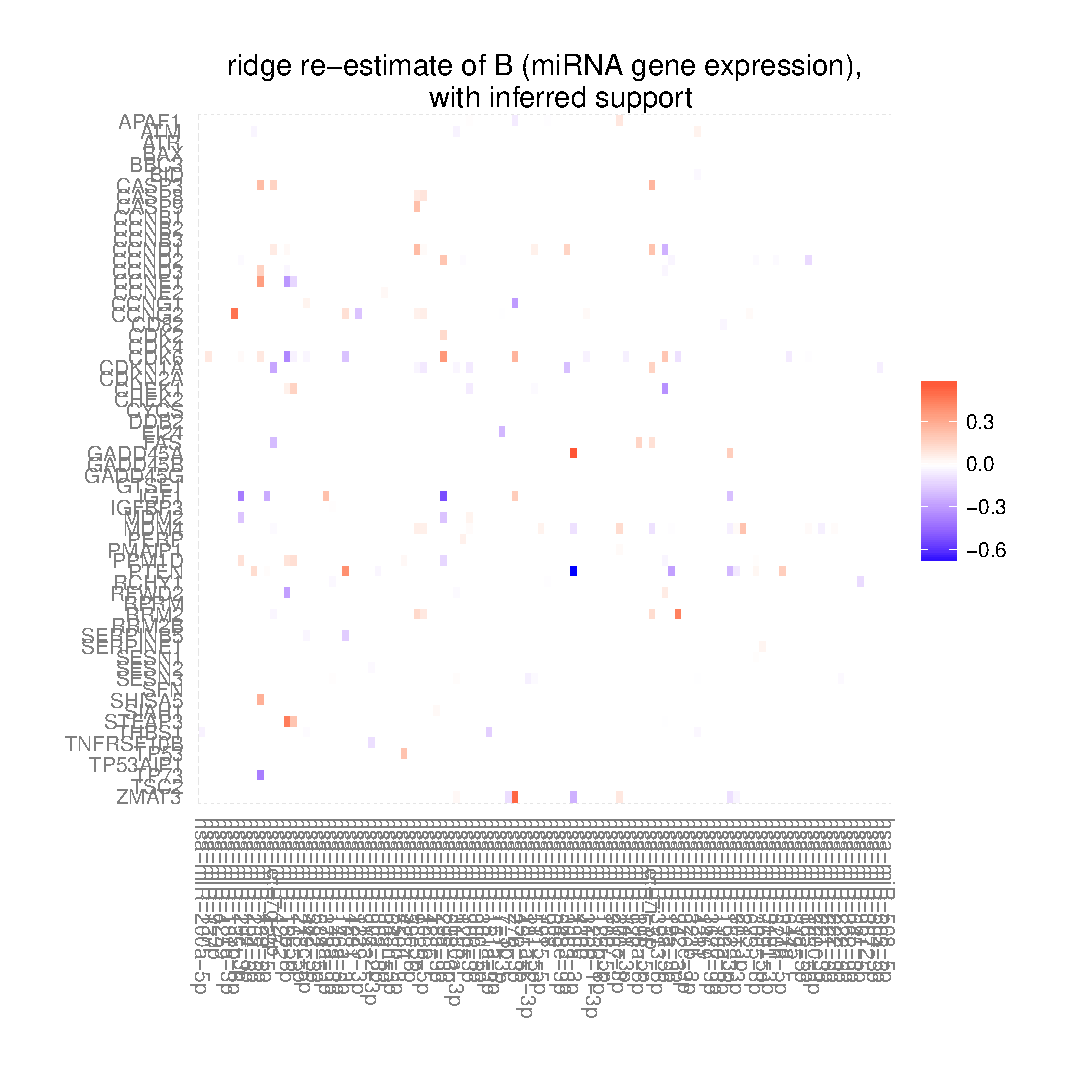
\includegraphics[scale=0.28]{Figure_16c.eps}
\end{tabular}
\caption{Heatmaps of the sparse re-estimated VARX(1) model parameters. Left panel: Estimates of $\mathbf{A}$, representing the temporal relations among mRNAs. Central panel and right panel show the estimate of $\mathbf{B}$, partitioned by molecular level (DNA copy number and miRNA, respectively).}
\label{fig:VARXestimatAandB}
\end{figure}



\begin{figure}[h!]
\centering
\begin{tabular}{c}
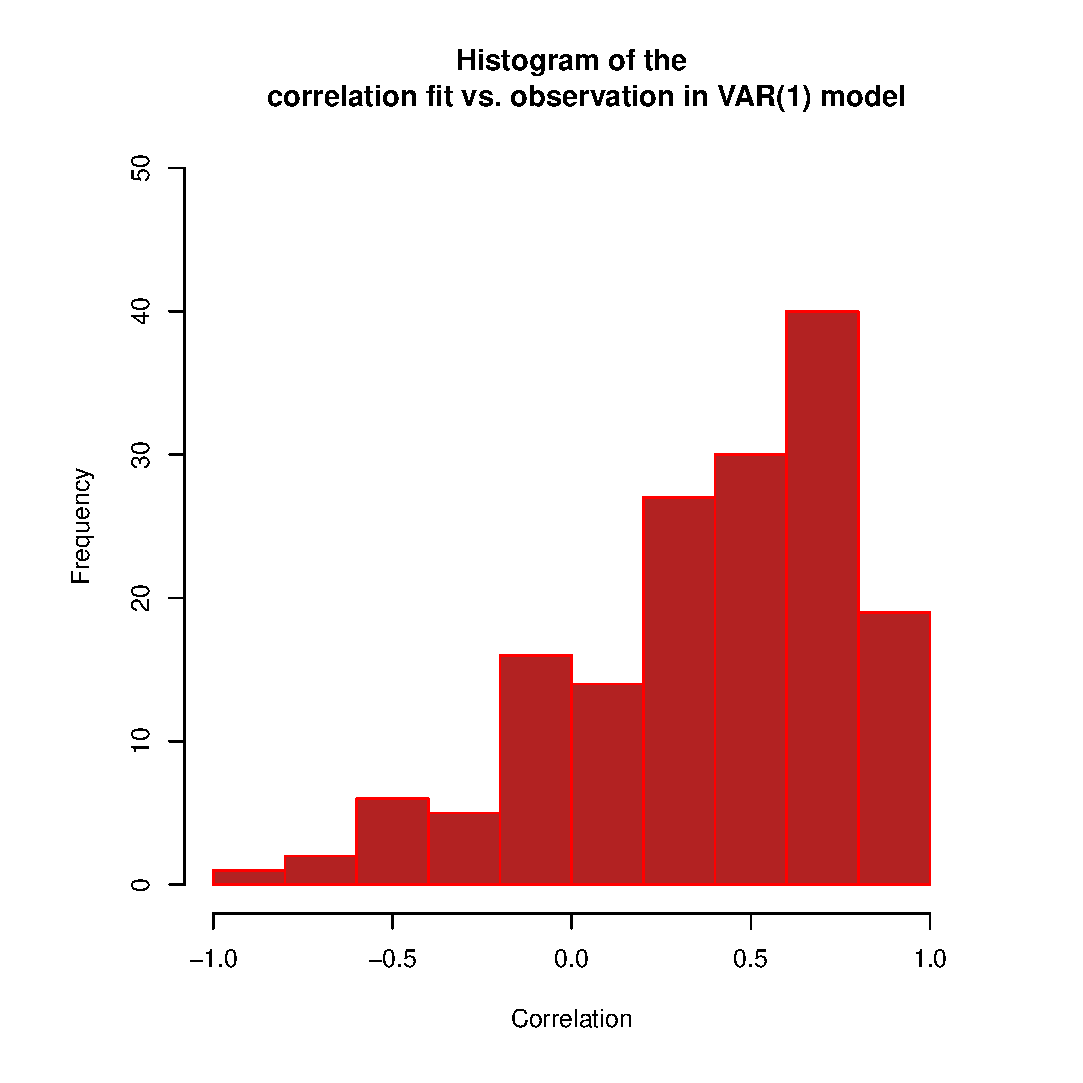
\includegraphics[scale=0.4]{Figure_13a.eps}
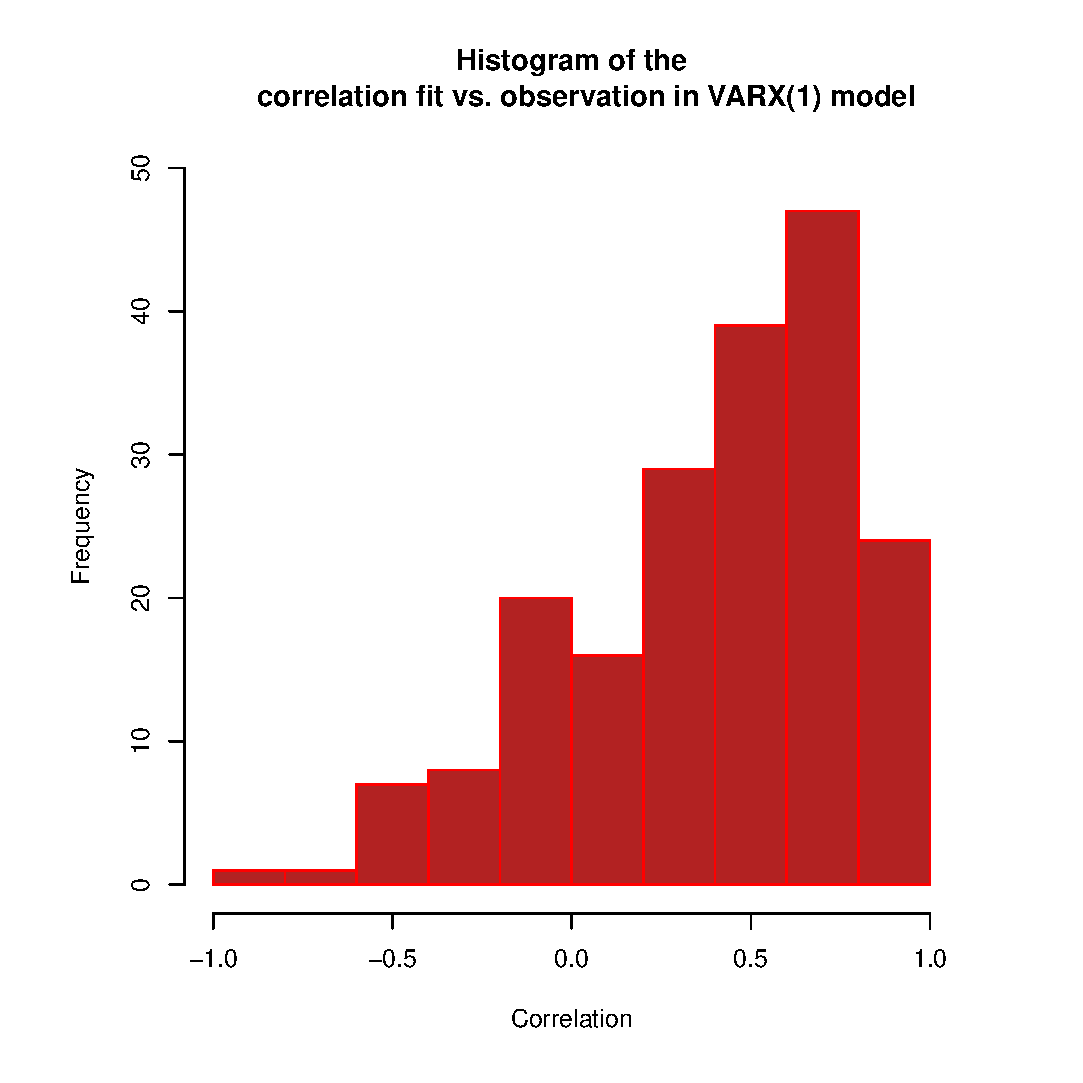
\includegraphics[scale=0.4]{Figure_13b.eps}
\end{tabular}
\caption{Histograms of Spearman correlations between the observations and VAR(1) and VARX(1) model fits (left and right panel, respectively).}
\label{fig:compareVAR1-VARX1}  
\end{figure}
